\documentclass[../Languages.tex]{subfiles}

\begin{document}
\usec{Go}\label{sec:g}

\cd{Go} (often referred to as \cd{golang}) is a programming language
created at Google in 2009 by Robert Griesemer, Rob Pike, and Ken Thompson. It
is a compiled, statically typed language in the tradition of
\cd{sec:algol} and \cd{sec:c}, with garbage collection, limited
structural typing, memory safety features and CSP-style concurrent programming
features added. The compiler and other language tools originally developed by
Google are all free and open source.

\subsection{Influence}\label{sub:influence}

\begin{Figure}
  \centering
  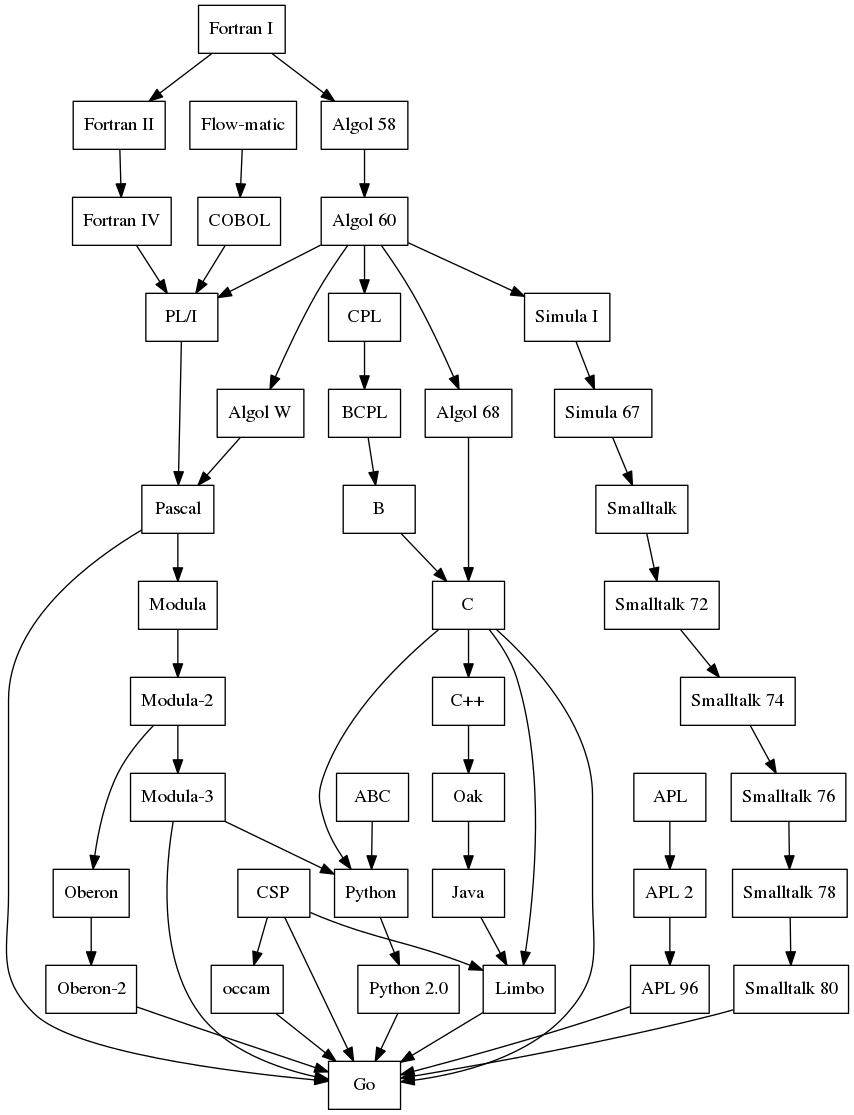
\includegraphics[height=0.5\textheight]{go}
  \captionof{figure}{Inheritance diagram for \cd{Go}.}
\end{Figure}

\newpage
\end{document}
